\section{Colored graphs and the bounded block}
\label{sec:blocks}

We now construct the metric space and anchors in \Cref{thm:blocks}.
The graphs below supply independently colored tree patterns in the empirical
limit. We join their
disjoint union through finitely many anchors, making the resulting space
bounded while keeping the small balls used to count support transitions
inside the source graphs. The lower bound for finite-rank operators will
use this local limit together with the properties in \Cref{lem:block-geometry}.

We first fix the graph conventions. Multiple edges are distinct edge
instances. Each instance has two oriented incidences $e,\bar e$, exchanged
by reversal, even when the edge is a loop. Thus a loop contributes two to
the degree. Write $e:x\to y$ when $x$ and $y$ are the initial and terminal
vertices, and let $\mathcal D(x)$ be the set of outgoing incidences at $x$.
A walk is \emph{nonbacktracking} if it never immediately takes the reverse
incidence of its preceding step. It may revisit vertices or take the same
loop incidence again. Graph distance uses unit edge lengths. A rooted
radius-$r$ ball is the induced multigraph on vertices at graph distance at
most $r$ from the root; its isomorphism type retains the colors, loops, and
edge multiplicities. Throughout the construction, only vertices are points
of the metric spaces: edge interiors are not included.

\subsection{A deterministic sequence with a colored tree limit}

We use the independent-permutation multigraph model described by Friedman
\cite[\S1, p.~2]{Friedman04}, in the empirical rooted-neighborhood viewpoint
of Benjamini and Schramm \cite[\S1.2]{BenjaminiSchramm01}. The precise colored
limit and deterministic selection needed here follow from the elementary
exploration argument below; no spectral estimate is used.

\begin{lemma}\label{lem:local-limit}
For every even integer $\Delta\ge4$ and positive integer $k$, there is a
deterministic sequence of nonempty finite $\Delta$-regular multigraphs
$G_m$, with vertices colored by $\{1,\ldots,k\}$, such that, for every
fixed integer $r\ge0$ and every possible induced rooted colored
radius-$r$ type $\tau$, the fraction of vertices of $G_m$ whose ball has
type $\tau$ converges to the probability of $\tau$ for the
$\Delta$-regular tree with independent uniform vertex colors.
\end{lemma}

\begin{proof}
On a vertex set of size $N$, choose $\Delta/2$ independent uniform
permutations $\sigma_1,\ldots,\sigma_{\Delta/2}$. For each pair $(a,v)$,
create a distinct undirected edge instance joining $v$ to $\sigma_a(v)$.
For each $a$, every vertex has one incidence directed to its image and
one directed to its preimage. A fixed point gives a loop with these two
incidences, and a permutation 2-cycle gives two parallel edge instances.
The resulting multigraph is therefore exactly $\Delta$-regular. Assign
independent uniform colors in $\{1,\ldots,k\}$ to its vertices, independently
of the permutations.

Fix $r\ge0$. Explore from a prescribed root in breadth-first order, revealing
every permutation image and inverse image at each vertex discovered at
distance at most $r$. Record newly discovered vertices at distance $r+1$
without expanding them. This extra layer reveals every edge of the induced
radius-$r$ ball, including edges between boundary vertices. The number of
queries and discovered vertices is bounded by a constant $C=C(\Delta,r)$,
independent of $N$.

Conditional on all revelations so far, the unrevealed part of each
permutation is a uniform bijection between its unused domains and ranges.
A query already exposed reuses its edge instance. A genuinely unexposed
image or inverse image is uniform among at least $N-C$ unused possibilities,
at most $C$ of which are previously discovered vertices. Its conditional
probability of such a collision is at most $C/(N-C)$ when $N>C$.
Before a collision, each fresh query adds one vertex and one edge to the
exploration tree; reused queries add nothing. In particular, a loop or a
second parallel edge is detected when its fresh query hits a known vertex.
A union bound over the queries makes the probability of any collision at
most $C^2/(N-C)=O_{\Delta,r}(N^{-1})$. Outside this event the induced
radius-$r$ ball is the regular-tree ball.

For two distinct prescribed roots, put both in the initially discovered
set and perform the two explorations together. With a larger constant
$C(\Delta,r)$, the same bound applies, counting a hit on either exploration
as a collision. With probability tending to one, the two induced
radius-$r$ balls are disjoint tree balls. These events concern only the
permutations, so the colors on all their distinct vertices remain
independent and uniform.

For a rooted radius-$r$ colored type $\tau$, let $I_v$ indicate that the
ball at $v$ has type $\tau$, and write
\[
 X_{\tau,N}=\frac1N\sum_v I_v,
 \qquad q_\tau=\Pp(\text{the colored tree ball has type }\tau).
\]
The one-root exploration gives $\E X_{\tau,N}\to q_\tau$. By exchangeability
and the two-root exploration,
\[
 \E X_{\tau,N}^2
 =\frac1N\E I_1+\left(1-\frac1N\right)\E(I_1I_2)
 \longrightarrow q_\tau^2.
\]
This also covers non-tree types, for which $q_\tau=0$. Consequently
$\operatorname{Var}(X_{\tau,N})\to0$, and each frequency converges in
probability to $q_\tau$.

For each $m\ge1$ there are only finitely many possible colored types at
radii at most $m$: bounded degree bounds the number of vertices and edge
instances in each ball, and the color set is finite. Convergence in
probability and a finite union bound show that, for all sufficiently large
$N$, with positive probability every one of these frequencies differs from
its tree probability by less than $1/m$. Choose such a realization with
$N=N_m$ strictly increasing in $m$. For each fixed radius and type the error
then tends to zero, which is the asserted deterministic convergence.
\end{proof}

\subsection{Labels, anchors, and the metric}

Fix an integer $p\ge1$. We choose the metric scales to meet two requirements
of the obstruction. Scalar tests taking values in $[-L,L]$ automatically
satisfy the Lipschitz inequality for opposing values at points separated by
at least $2L$. We make the source-to-anchor attachment length $R$ larger
than $2L$, so paths short enough to require further control cannot cross an
attachment edge. The later operator comparison across an attachment has
norm error at most $2pR+1$. Testing that comparison against a label bump
with Lipschitz constant at most $L/K$ incurs a loss of at most
$L(2pR+1)/K$, which must be small compared with its height $L$.
Set
\begin{equation}\label{eq:parameters}
 \begin{gathered}
 L=10p,\qquad R=3L=30p=:R_p,\qquad K=10p(R+1),\\
 D=K+2L+5,\qquad B=4R+D,\qquad V=1+4pB.
 \end{gathered}
\end{equation}
Substitution gives $B=300p^2+150p+5=B_p$. These metric scales satisfy
$R>2L$, $(2pR+1)/K\le1/5$, and $K+2L+1=D-4<D$. The label coordinates
will be capped at $D$. The last inequality leaves room for a label distance
below $K$, one source-edge step, and one support step of length at most
$2L$, while still keeping the relevant coordinate below the cap.

The degree and the number of colors serve different purposes. The
signed-measure argument will bound total variation by $V=1+4pB$; choosing
a large degree dilutes the loss from at most one exceptional direction per
support point. Choose an even integer $\Delta\ge4$ with $V/\Delta<1/20$,
and put
\[
 Q=\Delta^{2L+1},\qquad H=\Delta^{D+1}.
\]
The geometry below gives at most $Q$ nearby successors for a support point
and at most $H$ label coordinates below the cap, which will bound the
possible source colors for that point. A source walk itself has at most
$\Delta$ choices at each step. Thus larger degree helps the averaging
argument but also increases the number of walks in the matching estimate.
After fixing $\Delta$, choose an integer $k>2\Delta QH$, so that the
combined matching factor $\Delta QH/k$ is less than $1/2$. All these
choices are possible because the preceding quantities are finite.
Fix a deterministic sequence $(G_m)_{m\ge1}$ from
\Cref{lem:local-limit} for this $\Delta$ and $k$. All constants and the
entire sequence are now fixed, before any operator is considered.

Take disjoint copies of the graphs $G_m$, whose vertices we call
\emph{source vertices}. For a source vertex $x\in G_m$, define
$h(x)\in\{0,\ldots,D\}^k$ by
\[
 h_i(x)=\min\bigl\{D,\dist_{G_m}(x,\{\text{vertices of color }i\})\bigr\}
 \qquad(1\le i\le k).
\]
The distance is $+\infty$ if no vertex of color $i$ lies in the component
of $x$, so the corresponding coordinate is $D$. These labels are defined
using the unit graph distances, before the metric space below is formed.

Let $\mathcal H\subseteq\{0,\ldots,D\}^k$ be the set of labels realized by
all source vertices. For each $v\in\mathcal H$, add one new vertex $a_v$,
called an \emph{anchor}, with label $h(a_v)=v$. Set
$A_p=\{a_v:v\in\mathcal H\}$ and $a(x)=a_{h(x)}$. Join each source vertex
$x$ to $a(x)$ by an edge of length $R$. Join distinct anchors $a_v,a_w$
by an edge of length $2R+\norm{v-w}_\infty$. Retain every source graph edge
with length one. Let $M_p$ be the set of all source vertices and anchors,
and let $d_p(u,v)$ be the infimum of lengths of finite paths joining $u$
to $v$ in this weighted graph, allowing the zero-edge path when $u=v$.
Choose any anchor $o$ as basepoint; an anchor exists because every $G_m$ is
nonempty. \Cref{fig:anchors} shows how vertices sharing a label use one anchor.

\begin{figure}[ht]
\centering
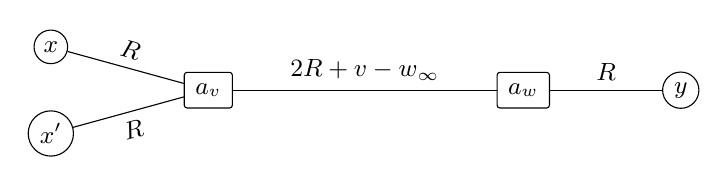
\begin{tikzpicture}[every node/.style={font=\small}]
 \node[circle,draw,inner sep=2pt] (x) at (0,0.55) {$x$};
 \node[circle,draw,inner sep=2pt] (xx) at (0,-0.55) {$x'$};
 \node[draw,rounded corners=1pt,inner sep=4pt] (a) at (2,0) {$a_v$};
 \node[draw,rounded corners=1pt,inner sep=4pt] (b) at (6,0) {$a_w$};
 \node[circle,draw,inner sep=2pt] (y) at (8,0) {$y$};
 \draw (x) -- node[above,sloped] {$R$} (a);
 \draw (xx) -- node[below,sloped] {$R$} (a);
 \draw (a) -- node[above] {$2R+\norm{v-w}_\infty$} (b);
 \draw (b) -- node[above] {$R$} (y);
\end{tikzpicture}
\caption{The added edges when $x,x'$ share label $v$ and $y$ has a different
label $w$.
The source vertices may belong to different graphs. Lines represent weighted
edges between vertices; their interiors are not points of $M_p$. Routes
through anchors can shorten long distances within a source graph.}
\label{fig:anchors}
\end{figure}

\begin{lemma}\label{lem:block-geometry}
The preceding construction has the following properties.
\begin{enumerate}[label=\textup{(\roman*)}]
\item $(M_p,d_p,o)$ is a countably infinite pointed metric space with
separation at least one and diameter at most $B=B_p$. The anchor set $A_p$
is finite and contains $o$. Each source edge has endpoints at $d_p$-distance
at most one.
\item The label map $h:M_p\to\{0,\ldots,D\}^k$ is 1-Lipschitz for the
sup norm. If a source vertex $x$ has color $i$, then $h_i(x)=0$, and
$h(a(x))=h(x)$.
\item For every source vertex $x$ and every anchor $a$,
\[
 d_p(x,a)\ge R=R_p,\qquad d_p(x,a(x))=R.
\]
In particular, $d_p(x,o)\ge R_p=30p$.
\item Every closed $d_p$-ball of radius $2L$ has at most $Q$ points.
For every $t\in M_p$, at most $H$ coordinates of $h(t)$ are strictly
below $D$.
\end{enumerate}
\end{lemma}

\begin{proof}
There are at most $(D+1)^k$ possible labels, so $A_p$ is finite. The disjoint
union of the nonempty finite graphs is countably infinite, and adjoining
finitely many anchors preserves that cardinality. The added edges connect
all vertices. Every edge length is a positive integer: this is clear for
source and attachment edges, and the sup distance between two integer labels
is an integer. For distinct endpoints the lengths of connecting finite paths
therefore form a nonempty subset of the positive integers, which has a least
element. Thus the infimum defining $d_p$ is attained. Symmetry and the
triangle inequality follow from reversal and concatenation of paths, and
distinct points have distance at least one. This also justifies using a
shortest path despite the possible infinite degrees of anchors. A source edge
itself gives distance at most one between its endpoints; for a loop the
distance is zero.

The sup distance between any two labels is at most $D$. Two source vertices
with different anchors can be joined by their two attachment edges and one
anchor edge, with total length at most
\[
 R+(2R+D)+R=4R+D=B.
\]
If their anchors agree, the route through that single anchor has length
$2R$. A source vertex and an anchor have distance at most $3R+D$, and two
anchors have distance at most $2R+D$, with the coincident-anchor cases
shorter. These bounds prove the diameter assertion. Any path from a source
vertex to an anchor must enter the anchor set for the first time along an
attachment edge of length $R$. Hence $d_p(x,a)\ge R$ for every anchor $a$.
The edge from $x$ to $a(x)$ realizes length $R$, proving (iii).

Across a source edge, the distances to a fixed color class differ by at most
one whenever that color is present in the component: append the edge to a
path realizing either distance. Capping at $D$ preserves this bound. If the
color is absent from the component, both coordinates are $D$. Thus adjacent
source labels have sup distance at most one. Labels agree across an
attachment edge, while each anchor edge has length at least the sup distance
between its endpoint labels. Summing these inequalities along any path gives
\[
 \norm{h(u)-h(v)}_\infty\le d_p(u,v).
\]
The own-color coordinate is zero by its definition, and anchor labels were
copied from their assigned vertices. This proves (ii), including paths that
use anchor shortcuts.

Every added edge has length at least $R=3L>2L$. A shortest path of length at
most $2L$ therefore uses only source edges. The closed radius-$2L$ ball about
an anchor is a singleton, and that about a source vertex is contained in its
radius-$2L$ ball in its own source graph. In a $\Delta$-regular multigraph, every vertex
at graph distance at most $s$ is reached by a walk of some length at most
$s$, and there are at most $\Delta^t$ walks of length $t$ from a fixed
vertex. Loops, parallel edges, and repeated vertices may cause several counted
walks to reach the same vertex. Therefore every such metric ball has at most
\[
 \sum_{t=0}^{2L}\Delta^t\le\Delta^{2L+1}=Q
\]
points. The inequality follows from the geometric sum formula and
$\Delta\ge2$.

Finally, if $h_i(x)<D$ at a source vertex, its integer graph distance to a
vertex of color $i$ is at most $D-1$. Witnesses for distinct colors are
distinct vertices, so the number of such coordinates is at most
\[
 \sum_{t=0}^{D-1}\Delta^t\le\Delta^{D+1}=H.
\]
Every anchor copies a source label, giving the same bound at all points of
$M_p$. This proves (iv).
\end{proof}

Part (iii) also gives a direct geometric proof that the wedge in
\Cref{sec:reduction} is unbounded. Each block contains a source vertex,
and the wedge preserves its distance from the common basepoint, which is
at least $R_p=30p$.

The construction has now fixed $M_p$, its finite anchor set, and the entire
graph sequence independently of any operator. The ball bound gives at most
$Q$ nearby successors for any point in any eventual finite support. The
label bound gives a second restriction: if a source vertex $x$ has color
$i$ and $\norm{h(x)-h(t)}_\infty<D$, then $h_i(t)<D$ because $h_i(x)=0$.
For each fixed $t$, proximity of labels therefore permits at most $H$
source colors. Both restrictions hold for every possible support, including
one containing anchors or vertices from several source graphs.
